\documentclass[a4paper,twocolumn]{article} % Document type

\ifx\pdfoutput\undefined
    %Use old Latex if PDFLatex does not work
   \usepackage[dvips]{graphicx}% To get graphics working
   \DeclareGraphicsExtensions{.eps} % Encapsulated PostScript
 \else
    %Use PDFLatex
   \usepackage[pdftex]{graphicx}% To get graphics working
   \DeclareGraphicsExtensions{.pdf,.jpg,.png,.mps} % Portable Document Format, Joint Photographic Experts Group, Portable Network Graphics, MetaPost
   \pdfcompresslevel=9
\fi
\usepackage{amsmath}
\usepackage{cleveref}
\usepackage{amsmath,amssymb}   % Contains mathematical symbols
\usepackage[ansinew]{inputenc} % Input encoding, identical to Windows 1252
\usepackage[english]{babel}    % Language
%\usepackage[round,authoryear]{natbib}  %Nice author (year) citations
\usepackage[square,numbers]{natbib}     %Nice numbered citations
%\bibliographystyle{unsrtnat}           %Unsorted bibliography
\bibliographystyle{plainnat}            %Sorted bibliography

\addtolength{\topmargin}{-30mm}% Removes 30mm from the top margin
\addtolength{\textheight}{30mm}% Adds it to the text height


\begin{document}

\section{Problem 2}
\label{sec:prob2} 
When 
$a=3,$ $b=f=-1,$ and $d=2,$
  we can obtain the differential equations as \cref{eqn:PPSystem1,eqn:PPSystem2}\par 
\begin{subequations}\label{eqn:PPSystem}
\begin{align}
    \dot{x} = x(3-x+cy) \label{eqn:PPSystem1} \\
    \dot{y} = y(2+ex-y) \label{eqn:PPSystem2}
\end{align}
\end{subequations}
The Jacobian matrix is defined as $A = \left. \frac{\partial\textbf{f}}{\partial \textbf{x}}(\textbf{x}) \right|_{\textbf{x}=\textbf{x}_0}$. The Jacobian matrix is calculated to be
\begin{equation*}
    \frac{\partial\textbf{f}}{\partial \textbf{x}}(\textbf{x}) =
    \left[\begin{array}{cc}
    3-2x+cy & cx \\
    ey & 2+ex-2y
    \end{array}\right],
\end{equation*}
\subsection{(c,e)=(-2,-1)}
%(-2,-1)
When $(c,e)=(-2,-1)$, the Jacobian matrix can be written as
\begin{equation*}
    \frac{\partial\textbf{f}}{\partial \textbf{x}}(\textbf{x}) =
    \left[\begin{array}{cc}
    3-2x-2y & -2x \\
    -y & 2-x-2y
    \end{array}\right],
\end{equation*}
There are four equilibrium points $(x^*,y^*)$ in total. They are $(0,0),(0,2),(3,0)$and$(1,1)$ respectively. The Jocabian matrix in this case is
\begin{equation*}
    A_{(0,0)} =
    \left[\begin{array}{cc}
    3 & 0 \\
    0 & 2
    \end{array}\right], \; A_{(0,2)} =
    \left[\begin{array}{cc}
    -1 & 0 \\
    -2 & -2
    \end{array}\right],   
    \end{equation*}
    \begin{equation*}
    A_{(3,0)} =
    \left[\begin{array}{cc}
    -3 & -6 \\
    0 & -1
    \end{array}\right], \;A_{(1,1)} =
    \left[\begin{array}{cc}
    -1 & -2 \\
    -1 & -1
    \end{array}\right].
\end{equation*}
The eigenvalues of the Jacobian matrix are given by the characteristic equation
\begin{equation*}
    \det(\lambda I - A) = 0.
\end{equation*}
The characteristic equation of the system linearized around \mbox{(0,0)} is
\begin{equation*}
    \lambda^2 -5 \lambda + 6 = 0,
\end{equation*}
which gives the eigenvalues $\lambda_{1} = 3$ and $\lambda_{2} = 2$. The equilibrium $(0,0)$ is an unstable node. 
The characteristic equation of the system linearized around \mbox{(0,2)} is
\begin{equation*}
    \lambda^2 +3 \lambda + 2 = 0,
\end{equation*}
which gives the eigenvalues $\lambda_1 = -1$ and $\lambda_2 = -2$. The equilibrium $(0,2)$ is a stable node. 
The characteristic equation of the system linearized around \mbox{(3,0)} is
\begin{equation*}
    \lambda^2 +4 \lambda + 3 = 0,
\end{equation*}
which gives the eigenvalues $\lambda_1 = -1$ and $\lambda_2 = -3$. The equilibrium $(3,0)$ is a stable node.
The characteristic equation of the system linearized around \mbox{(1,1)} is
\begin{equation*}
    \lambda^2 +2 \lambda - 1 = 0,
\end{equation*}
which gives the eigenvalues $\lambda_1 = \sqrt{2} -1 \approx 0.414$ and $\lambda_2 = -1 -\sqrt{2} \approx -2.414$. The equilibrium $(1,1)$ is a saddle point.


In this case, the relationship between $x$ and $y$ is competitive. This implies that one species would always tend to become dominate and the other would become extinct based on the initial ratio. There is one point where two species could co-exist but it$'$s not stable since the equilibrium could be broken easily as long as small number disturbance happens.  

\subsection{(c,e)=(-2,1)}
%(-2,1)
When $(c,e)=(-2,1)$, the Jacobian matrix can be written as
\begin{equation*}
    \frac{\partial\textbf{f}}{\partial \textbf{x}}(\textbf{x}) =
    \left[\begin{array}{cc}
    3-2x-2y & -2x \\
    y & 2+x-2y
    \end{array}\right],
\end{equation*}
There are three equilibrium points $(x^*,y^*)$ in total. They are $(0,0),(0,2)$ and $(3,0)$ respectively. The Jocabian matrix in this case is
\begin{equation*}
    A_{(0,0)} =
    \left[\begin{array}{cc}
    3 & 0 \\
    0 & 2
    \end{array}\right], \; A_{(0,2)} =
    \left[\begin{array}{cc}
    -1 & 0 \\
    2 & -2
    \end{array}\right],   
    \end{equation*}
    \begin{equation*}
    A_{(3,0)} =
    \left[\begin{array}{cc}
    -3 & -6 \\
    0 & 5
    \end{array}\right].
\end{equation*}
The eigenvalues of the Jacobian matrix are given by the characteristic equation
\begin{equation*}
    \det(\lambda I - A) = 0.
\end{equation*}
The characteristic equation of the system linearized around \mbox{(0,0)} is
\begin{equation*}
    \lambda^2 -5 \lambda + 6 = 0,
\end{equation*}
which gives the eigenvalues $\lambda_{1} = 3$ and $\lambda_{2} = 2$. The equilibrium $(0,0)$ is an unstable node. 
The characteristic equation of the system linearized around \mbox{(0,2)} is
\begin{equation*}
    \lambda^2 +3 \lambda + 2 = 0,
\end{equation*}
which gives the eigenvalues $\lambda_1 = -1$ and $\lambda_2 = -2$. The equilibrium $(0,2)$ is a stable node. 
The characteristic equation of the system linearized around \mbox{(3,0)} is
\begin{equation*}
    \lambda^2 -2 \lambda - 15 = 0,
\end{equation*}
which gives the eigenvalues $\lambda_1 = -3$ and $\lambda_2 = 5$. The equilibrium $(3,0)$ is a saddle point.


In this case, the relationship between the two species is $y$ preying on $x$. This implies that $y$ would increase if the relative amount of $x$ is huge and vice versa.

\subsection{(c,e)=(2,-1)}
%(2,-1)
When $(c,e)=(2,-1)$, the Jacobian matrix can be written as
\begin{equation*}
    \frac{\partial\textbf{f}}{\partial \textbf{x}}(\textbf{x}) =
    \left[\begin{array}{cc}
    3-2x+2y & 2x \\
    -y & 2-x-2y
    \end{array}\right],
\end{equation*}
There are three equilibrium points $(x^*,y^*)$ in total. They are $(0,0),(0,2)$ and $(3,0)$ respectively. The Jocabian matrix in this case is
\begin{equation*}
    A_{(0,0)} =
    \left[\begin{array}{cc}
    3 & 0 \\
    0 & 2
    \end{array}\right], \; A_{(0,2)} =
    \left[\begin{array}{cc}
    7 & 0 \\
    -2 & -2
    \end{array}\right],   
    \end{equation*}
    \begin{equation*}
    A_{(3,0)} =
    \left[\begin{array}{cc}
    -3 & 6 \\
    0 & -1
    \end{array}\right].
\end{equation*}
The eigenvalues of the Jacobian matrix are given by the characteristic equation
\begin{equation*}
    \det(\lambda I - A) = 0.
\end{equation*}
The characteristic equation of the system linearized around \mbox{(0,0)} is
\begin{equation*}
    \lambda^2 -5 \lambda + 6 = 0,
\end{equation*}
which gives the eigenvalues $\lambda_{1} = 3$ and $\lambda_{2} = 2$. The equilibrium $(0,0)$ is an unstable node. 
The characteristic equation of the system linearized around \mbox{(0,2)} is
\begin{equation*}
    \lambda^2 -5 \lambda - 14 = 0,
\end{equation*}
which gives the eigenvalues $\lambda_1 = -2$ and $\lambda_2 = 7$. The equilibrium $(0,2)$ is a saddle node. 
The characteristic equation of the system linearized around \mbox{(3,0)} is
\begin{equation*}
    \lambda^2 +4 \lambda + 3 = 0,
\end{equation*}
which gives the eigenvalues $\lambda_1 = -3$ and $\lambda_2 = -1$. The equilibrium $(3,0)$ is a stable point.


In this case, the relationship between the two species is $x$ preying on $y$. This implies that $x$ tends to increase if the relative amount of $y$ is huge and vice versa.   

\subsection{(c,e)=(2,1)} 
%(2,1)
When $(c,e)=(2,1)$, the Jacobian matrix can be written as
\begin{equation*}
    \frac{\partial\textbf{f}}{\partial \textbf{x}}(\textbf{x}) =
    \left[\begin{array}{cc}
    3-2x+2y & 2x \\
    y & 2+x-2y
    \end{array}\right],
\end{equation*}
There are three equilibrium points $(x^*,y^*)$ in total. They are $(0,0),(0,2)$ and $(3,0)$ respectively. The Jocabian matrix in this case is
\begin{equation*}
    A_{(0,0)} =
    \left[\begin{array}{cc}
    3 & 0 \\
    0 & 2
    \end{array}\right], \; A_{(0,2)} =
    \left[\begin{array}{cc}
    7 & 0 \\
    2 & -2
    \end{array}\right],   
    \end{equation*}
    \begin{equation*}
    A_{(3,0)} =
    \left[\begin{array}{cc}
    -3 & 6 \\
    0 & 5
    \end{array}\right].
\end{equation*}
The eigenvalues of the Jacobian matrix are given by the characteristic equation
\begin{equation*}
    \det(\lambda I - A) = 0.
\end{equation*}
The characteristic equation of the system linearized around \mbox{(0,0)} is
\begin{equation*}
    \lambda^2 -5 \lambda + 6 = 0,
\end{equation*}
which gives the eigenvalues $\lambda_{1} = 3$ and $\lambda_{2} = 2$. The equilibrium $(0,0)$ is an unstable node. 
The characteristic equation of the system linearized around \mbox{(0,2)} is
\begin{equation*}
    \lambda^2 -5 \lambda - 14 = 0,
\end{equation*}
which gives the eigenvalues $\lambda_1 = -2$ and $\lambda_2 = 7$. The equilibrium $(0,2)$ is a saddle node. 
The characteristic equation of the system linearized around \mbox{(3,0)} is
\begin{equation*}
    \lambda^2 -2 \lambda - 15 = 0,
\end{equation*}
which gives the eigenvalues $\lambda_1 = -3$ and $\lambda_2 = 5$. The equilibrium $(3,0)$ is a saddle point.


In this case, the relationship between the two species is symbiotic. This implies that one species would increase if the other one increases. 

\section{Problem 3}
\label{sec:prob3} 
When 
$a=e=1$, $b=f=0$, and $c=d=-1$,
  we can obtain the differential equations as \cref{eqn:PPSystem1,eqn:PPSystem2}\par 
\begin{subequations}\label{eqn:PPSystem}
\begin{align}
    \dot{x} = x(1-y) \label{eqn:PPSystem1} \\
    \dot{y} = y(-1+x) \label{eqn:PPSystem2}
\end{align}
\end{subequations}
The Jacobian matrix is defined as $A = \left. \frac{\partial\textbf{f}}{\partial \textbf{x}}(\textbf{x}) \right|_{\textbf{x}=\textbf{x}_0}$. The Jacobian matrix is calculated to be
\begin{equation*}
    \frac{\partial\textbf{f}}{\partial \textbf{x}}(\textbf{x}) =
    \left[\begin{array}{cc}
    1-y & -x \\
    y & -1+x
    \end{array}\right],
\end{equation*}
By calculating $(x^*,y^*)$, the system has two equilibrium points $(0,0)$ and $(1,1)$.The Jocabian matrix in this case is
\begin{equation*}
    A_{(0,0)} =
    \left[\begin{array}{cc}
    1 & 0 \\
    0 & -1
    \end{array}\right], \; A_{(1,1)} =
    \left[\begin{array}{cc}
    0 & -1 \\
    1 & 0
    \end{array}\right],   
    \end{equation*}
 The characteristic equation of the system linearized around \mbox{(0,0)} is
\begin{equation*}
    \lambda^2 -1 = 0,
\end{equation*}
which gives the eigenvalues $\lambda_{1,2} = \pm 1$. The equilibrium $(0,0)$ is a saddle point. 
The characteristic equation of the system linearized around \mbox{(1,1)} is
\begin{equation*}
    \lambda^2 +1 = 0,
\end{equation*}
which gives the eigenvalues $\lambda_{1,2} = \pm j$. The equilibrium $(1,1)$ is a non-hyperbolic point so the stability needs to be checked with other methods. From the plot we can infer that this equilibrium is a stable point.    


\section{Problem 5}
\label{sec:prob5} 
When the number of species $N>2$, a general equation to express the population model can be deduced as~(\ref{eqn:p5}).
\begin{equation}\label{eqn:p5}
   \dot{x}_i = x_i(\alpha_i+ \sum_{j=1}^{N} \beta_{ij}x_j), ~i=1...N
\end{equation}
The coefficients $\beta_{ij}$ will be decided based on the relationship among species further. Intuitively, when $x_j$ preys on $x_i$, then $\beta_{ij}<0, \beta_{ji}>0$;when $x_i$ preys on $x_j$, then $\beta_{ij}>0, \beta_{ji}<0$;when $x_j$ and $x_i$ are competitive, then both $\beta_{ij}$ and $\beta_{ij}$ will be negative;when $x_j$ and $x_i$ are symbiotic, then both $\beta_{ij}$ and $\beta_{ij}$ will be positive;$\beta_{ij}$ and $\beta_{ji}$ might be zero if the relationship between $x_i$ and $x_j$ keeps unknown. 

\begin{figure*}[p] % The * makes the figure span both columns, p places the figure on a float page
  \begin{center}
    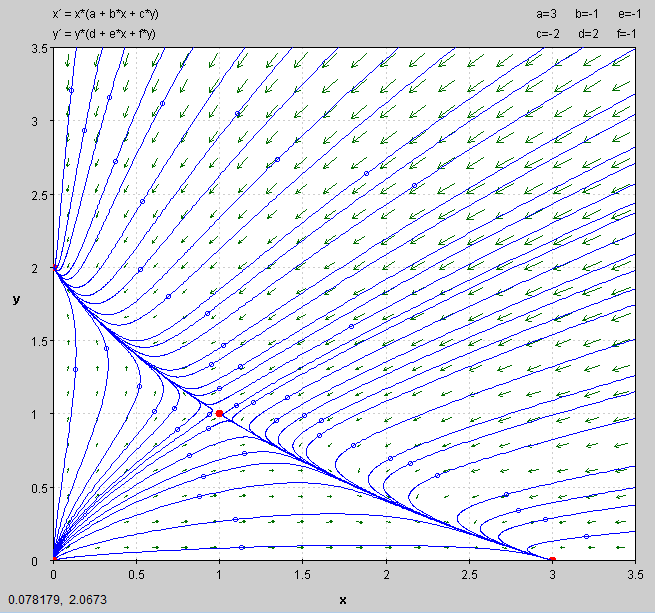
\includegraphics[width = 0.9\textwidth, height = 0.5\textwidth]{-2-1}
  \end{center}
  \caption{Phase portrait of the system in \eqref{eqn:PPSystem}, which has an unstable node at \mbox{(0,0)}, two stable points at \mbox{(0,2)} and \mbox{(3,0)} and a saddle point at \mbox{(1,1)}. All the equilibriums are marked by large dots and selected trajectories are marked by solid lines. This figure was generated using PPLANE (\texttt{http://math.rice.edu/~dfield/dfpp.html}).}
  \label{fig:pplane}
\end{figure*}

\begin{figure*}[p] % The * makes the figure span both columns, p places the figure on a float page
  \begin{center}
    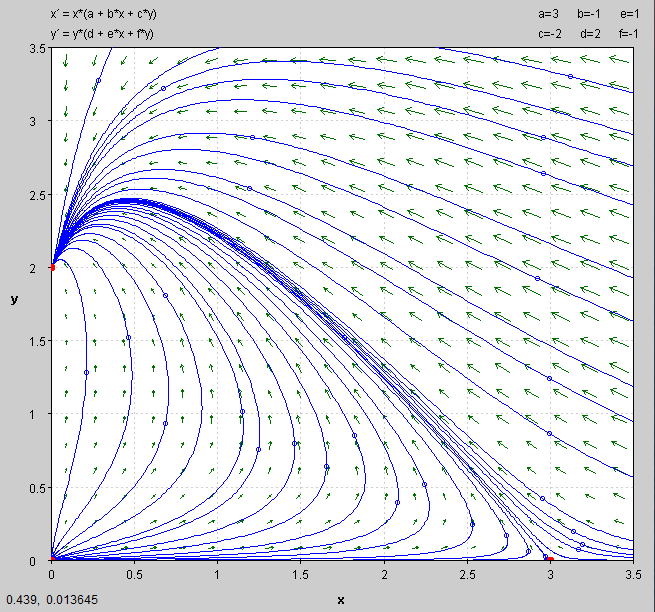
\includegraphics[width = 0.9\textwidth, height = 0.5\textwidth]{-21}
  \end{center}
  \caption{Phase portrait of the system in \eqref{eqn:PPSystem}, which has an unstable node at \mbox{(0,0)}, a stable point at \mbox{(0,2)} and a saddle at \mbox{(3,0)}. All the equilibriums are marked by large dots and selected trajectories are marked by solid lines. This figure was generated using PPLANE (\texttt{http://math.rice.edu/~dfield/dfpp.html}).}
  \label{fig:pplane2}
\end{figure*}

\begin{figure*}[p] % The * makes the figure span both columns, p places the figure on a float page
  \begin{center}
    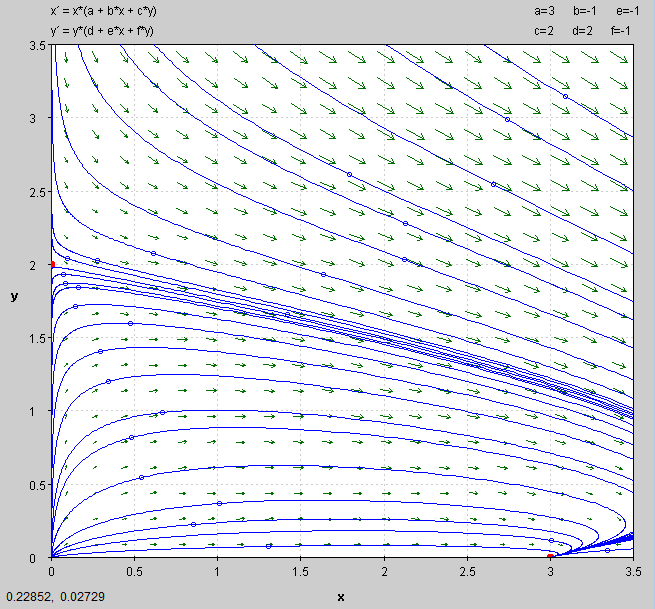
\includegraphics[width = 0.9\textwidth, height = 0.5\textwidth]{2-1}
  \end{center}
  \caption{Phase portrait of the system in \eqref{eqn:PPSystem}, which has an unstable node at \mbox{(0,0)}, a saddle point at \mbox{(0,2)} and a stable at \mbox{(3,0)}. All the equilibriums are marked by large dots and selected trajectories are marked by solid lines. This figure was generated using PPLANE (\texttt{http://math.rice.edu/~dfield/dfpp.html}).}
  \label{fig:pplane2}
\end{figure*}

\begin{figure*}[p] % The * makes the figure span both columns, p places the figure on a float page
  \begin{center}
    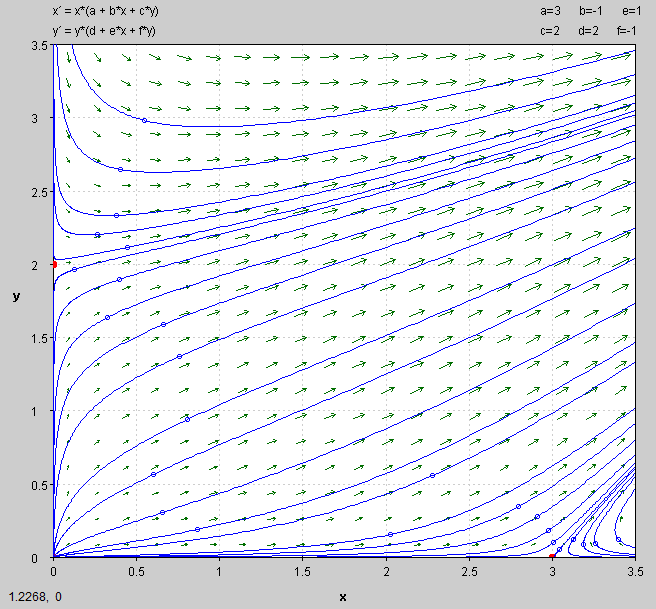
\includegraphics[width = 0.9\textwidth, height = 0.5\textwidth]{21}
  \end{center}
  \caption{Phase portrait of the system in \eqref{eqn:PPSystem}, which has an unstable node at \mbox{(0,0)}, two saddle points at \mbox{(0,2)} \mbox{(3,0)}. All the equilibriums are marked by large dots and selected trajectories are marked by solid lines. This figure was generated using PPLANE (\texttt{http://math.rice.edu/~dfield/dfpp.html}).}
  \label{fig:pplane2}
\end{figure*}

\begin{figure*}[p] % The * makes the figure span both columns, p places the figure on a float page
  \begin{center}
    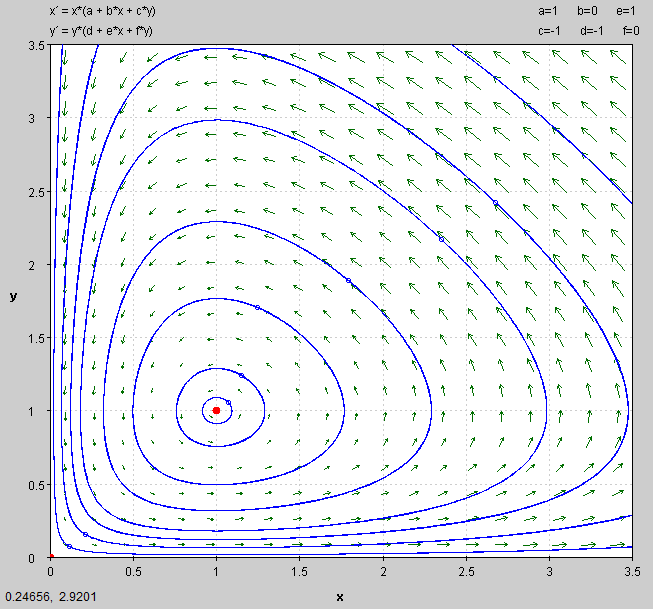
\includegraphics[width = 0.9\textwidth, height = 0.5\textwidth]{p3}
  \end{center}
  \caption{Phase portrait of the system in \eqref{eqn:PPSystem}, which has a saddle node at \mbox{(0,0)} and a stable point at \mbox{(1,1)}. All the equilibriums are marked by large dots and selected trajectories are marked by solid lines. This figure was generated using PPLANE (\texttt{http://math.rice.edu/~dfield/dfpp.html}).}
  \label{fig:pplane2}
\end{figure*}  
\end{document}